\documentclass[twocolumn]{article}
\usepackage{graphicx}
\usepackage{float}
\usepackage{lipsum}

\title{Enhancing household survey microdata accuracy using machine learning: project plan}
\date{}
\author{Nikhil Woodruff}

\begin{document}

\maketitle

\section{Project outline}

Tax-benefit policy is the set of rules that determine tax liabilities and benefit entitlements, deciding the allocation of nearly half of GDP in the United Kingdom alone. When policymakers, think-tanks or academic institutions propose changes to tax-benefit policy, they often use mathematical models to estimate the impact of such changes. The dominant approach to modelling tax-benefit policy is \emph{microsimulation}, a method composed of two parts: a model of policy logic that can compute taxes and benefits for a given household under current and proposed changes, and dataset representative of a target population, on which the policy model is executed. Most microsimulation models use a household survey dataset as their input. The most common of these surveys is the Family Resources Survey (FRS).

The accuracy of microsimulation models is crucial to their utility, and since policy logic is straightforward to verify (since the logic is specified explicitly in legislation), most microsimulation inaccuracy is due to the accuracy of the data. This project will center around the question of \emph{how much can computational methods improve the accuracy of household survey microdata}, predicated on three assumptions which can each be tested: that the unadjusted UK household survey data has poor accuracy for some questions, that existing methods to improve it distort the data (reducing its accuracy in some areas), and that machine learning-based approaches can significantly improve accuracy across most uses of the dataset. \emph{Accuracy} is not a particularly well-defined term, and for this project it is important, so I use the definition: a household survey's accuracy is the extent to which it gives answers to questions that are close to questions posed to the target population (here, the UK household population).

Broadly, the main problems with the FRS are that we know it is inaccurate for at least two groups: high incomes and benefit claimants - we know this because more robust surveys (administrative datasets) give substantially different answers to questions (for example, total budgetary imapcts of programs). The most common survey improvement techniques are designed to explicitly fix these issues directly (regardless of how they affect accuracy in other areas). These are \emph{percentile adjustment}, adjusting data values in order to make the distribution similar to that in another survey, and \emph{record matching}, replacing data values with that of the most similar record in another dataset. These techniques are designed to improve the accuracy of the FRS for high-income and benefit claimant households, but they are not designed to improve the accuracy of the FRS for other groups. This project will test the accuracy improvement of these methods against a process involving two alternatives: \emph{gradient descent-based reweighting} and \emph{random forest model-based imputation}. The former is a method of adjusting the weights of the FRS to make it more similar to another survey, while the latter is a method of imputing replacement values in the FRS using a random forest model trained on the FRS and another survey.

In order to assess these improvement methods, this project will create a computational method of estimating survey accuracy, which aggregates as many known sources of truth as possible (e.g. from census data and administrative statistics) and measures a survey dataset's deviation from each of these data.
\newpage
\section{Project plan}

The project has been split into several sections for simplicity. Each task, numbered below, is shown in the Gantt chart in Figure \ref{gantt_chart}.

\begin{enumerate}
    \item \textbf{Literature review} - review the literature on survey accuracy, survey improvement techniques, and machine learning methods for survey improvement.
    \item \textbf{Implement percentile adjustment} - implement a method of percentile adjustment in Python.
    \item \textbf{Implement record matching} - implement a method of record matching in Python between the FRS and Survey of Personal Incomes (HMRC administrative data).
    \item \textbf{Implement survey accuracy estimation} - implement the accuracy estimation function for the FRS, using UK administrative data points.
    \item \textbf{Implement gradient descent-based reweighting} - implement gradient descend-based reweighting in Python.
    \item \textbf{Implement random forest model-based imputation} - implement a method of random forest model-based imputation in Python.
    \item \textbf{Compare all three methods} - compare the accuracy of the three methods, and the accuracy of the FRS before and after each method.
    \item \textbf{Write up results} - write up the results of the project in a report.
    \item \textbf{Review report} - review the report.
\end{enumerate}

\begin{figure}
    \centering
    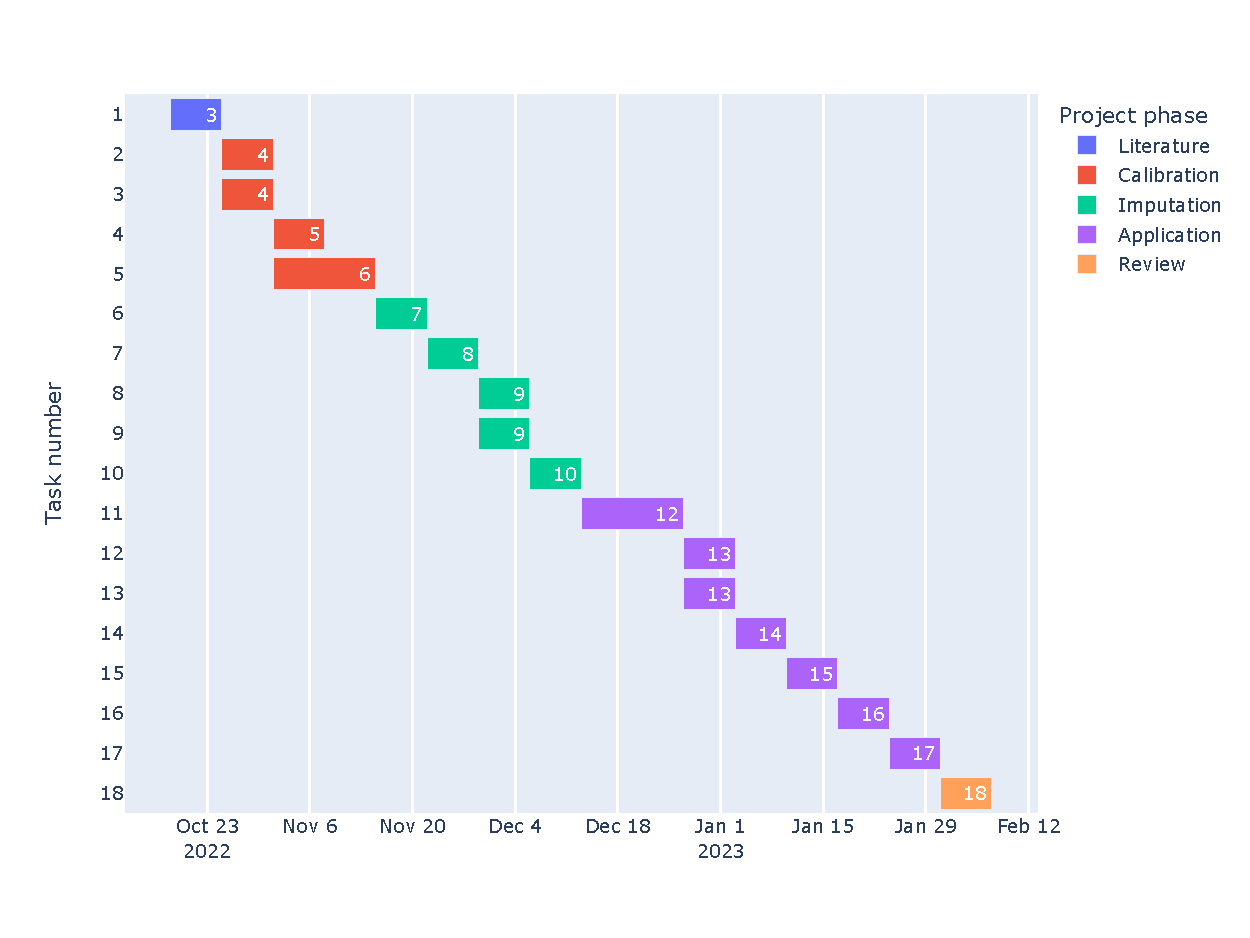
\includegraphics[width=0.5\textwidth]{gantt_chart.pdf}
    \caption{Gantt chart with project milestones}
    \label{gantt_chart}
\end{figure}

\end{document}
